\section{\our Step 1: Sensor Readings to TX Location Distributions}
\label{sec:translate}

In this section, we present the first step of our overall approach to the \mtl problem, i.e., 
the image-to-image translation step which translates/transforms the sensor reading to distributions
of TX locations. Here, we first create a grayscale image to represent the input sensor readings;
this image encodes both the sensors' RSS readings and the sensors' physical location. We then train and use
a convolutional neural network (CNN) model to transform this input image
to an output image which represents the distribution of TX locations. Pixels in the output image that have higher values will have a higher chance of having a TX being present at that location. 
 
\para{Input/Output Image Sizes and Tiling Approach for Large Areas.}
We need to represent data by images of certain sizes.
Typically, an image should be a size of a few hundred pixels by a few hundred pixels, since a thousand pixels by thousand pixels images will consume too much GPU memory.
In this chapter, we pick $100\times 100$ as the size for both our input and output images in the first image-to-image translation step.
Given an area that we want to monitor and a $100\times100$ size image, we will know how large an area a pixel will represent and we call it a pixel subarea.
%%%%%%%%
A large pixel subarea could certainly lead to high localization errors, due
to very coarse granularity. We can address this by using a ``tiling"
technique, wherein we divide the given area into tiles, then represent each 
tile by $100\times100$ size image and use our localization techniques in the tile.
We can do some post-processing to handle cross-tiling issues (e.g., \cite{icccn20-deeptxfinder} uses overlapping tiles and employs a voting scheme inside the overlapping tile area).
 
\eat{\blue{For our \our, each pixel represents a $10m\times 10m$ area. Since \our input image is of size $100\times 100$, the whole input image represents a $1000m\times1000m$ area. 
To deal with a larger area, let's say $10000m\times 10000m$ area, two simple methods are: increase the input image size to $1000\times 1000$; 
Or let each pixel represent a $100m\times 100m$ area.
The first method requires redesigning \our (changing layer hyperparameter etc.).
Note that the input image size is usually in the range of lower hundreds. 
For example, $224\times 224$ is used by ResNet \cite{resnet} and $416\times 416$ is used by YOLO. 
$1000\times 1000$ is generally speaking too big as it will consume too much GPU memory.
Also, a pixel representing a larger area means coarser granularity and lower accuracy.
A reasonable approach will be keeping the \our as it is, and use a ``sliding window" like method, i.e. slide the \our 100 times (10 rows, 10 columns) to cover the $10000m\times10000m$ area.
\deeptx\cite{icccn20-deeptxfinder} is using this idea and they name it a tile-based approach.
To deal with smaller areas, we can fill the rest of the area with noise floor values. 
By filling, we can make smaller images fit into the $100\times100$ input size requirement of \imgimg.
In the following subsection \ref{subsec:ipsn}, we demonstrate how we generate a $100\times 100$ size image from a $10\times 10$ size grid in real-world testbed data.}
}
%\todo[inline]{Is this 10m x 10m ?}


%%%%%%%%%%%%%%%%%%%%%%%%%%%%%%%%%%%%%%%%%%%

\subsection{Input Image Representing Sensors' Readings}

We localize transmitters based on observations from a set of sensors, i.e. solve the \mtl problem assuming only intruders.
%Below, we present details on how to represent the information gathered from the set of crowd-sourced sensors.
%\para{Sensor Observations' Matrix to Image.} 
The input of the localization method is sensor observations. 
Here, an {\em observation} at a sensor is the received power (RSS, in decibels) over a time window of a certain duration, in the frequency of interest (we assume only one wireless frequency). 
RSS is computed using FFT over the I/Q samples collected in a time window. More specifically, in our evaluations, we use a Python API \cite{psd} that computes the power spectral density from a sequence of signal data (I/Q samples), and then, we choose the RSS at the frequency of interest.
%%%%
\begin{figure}[t]
    \centering
    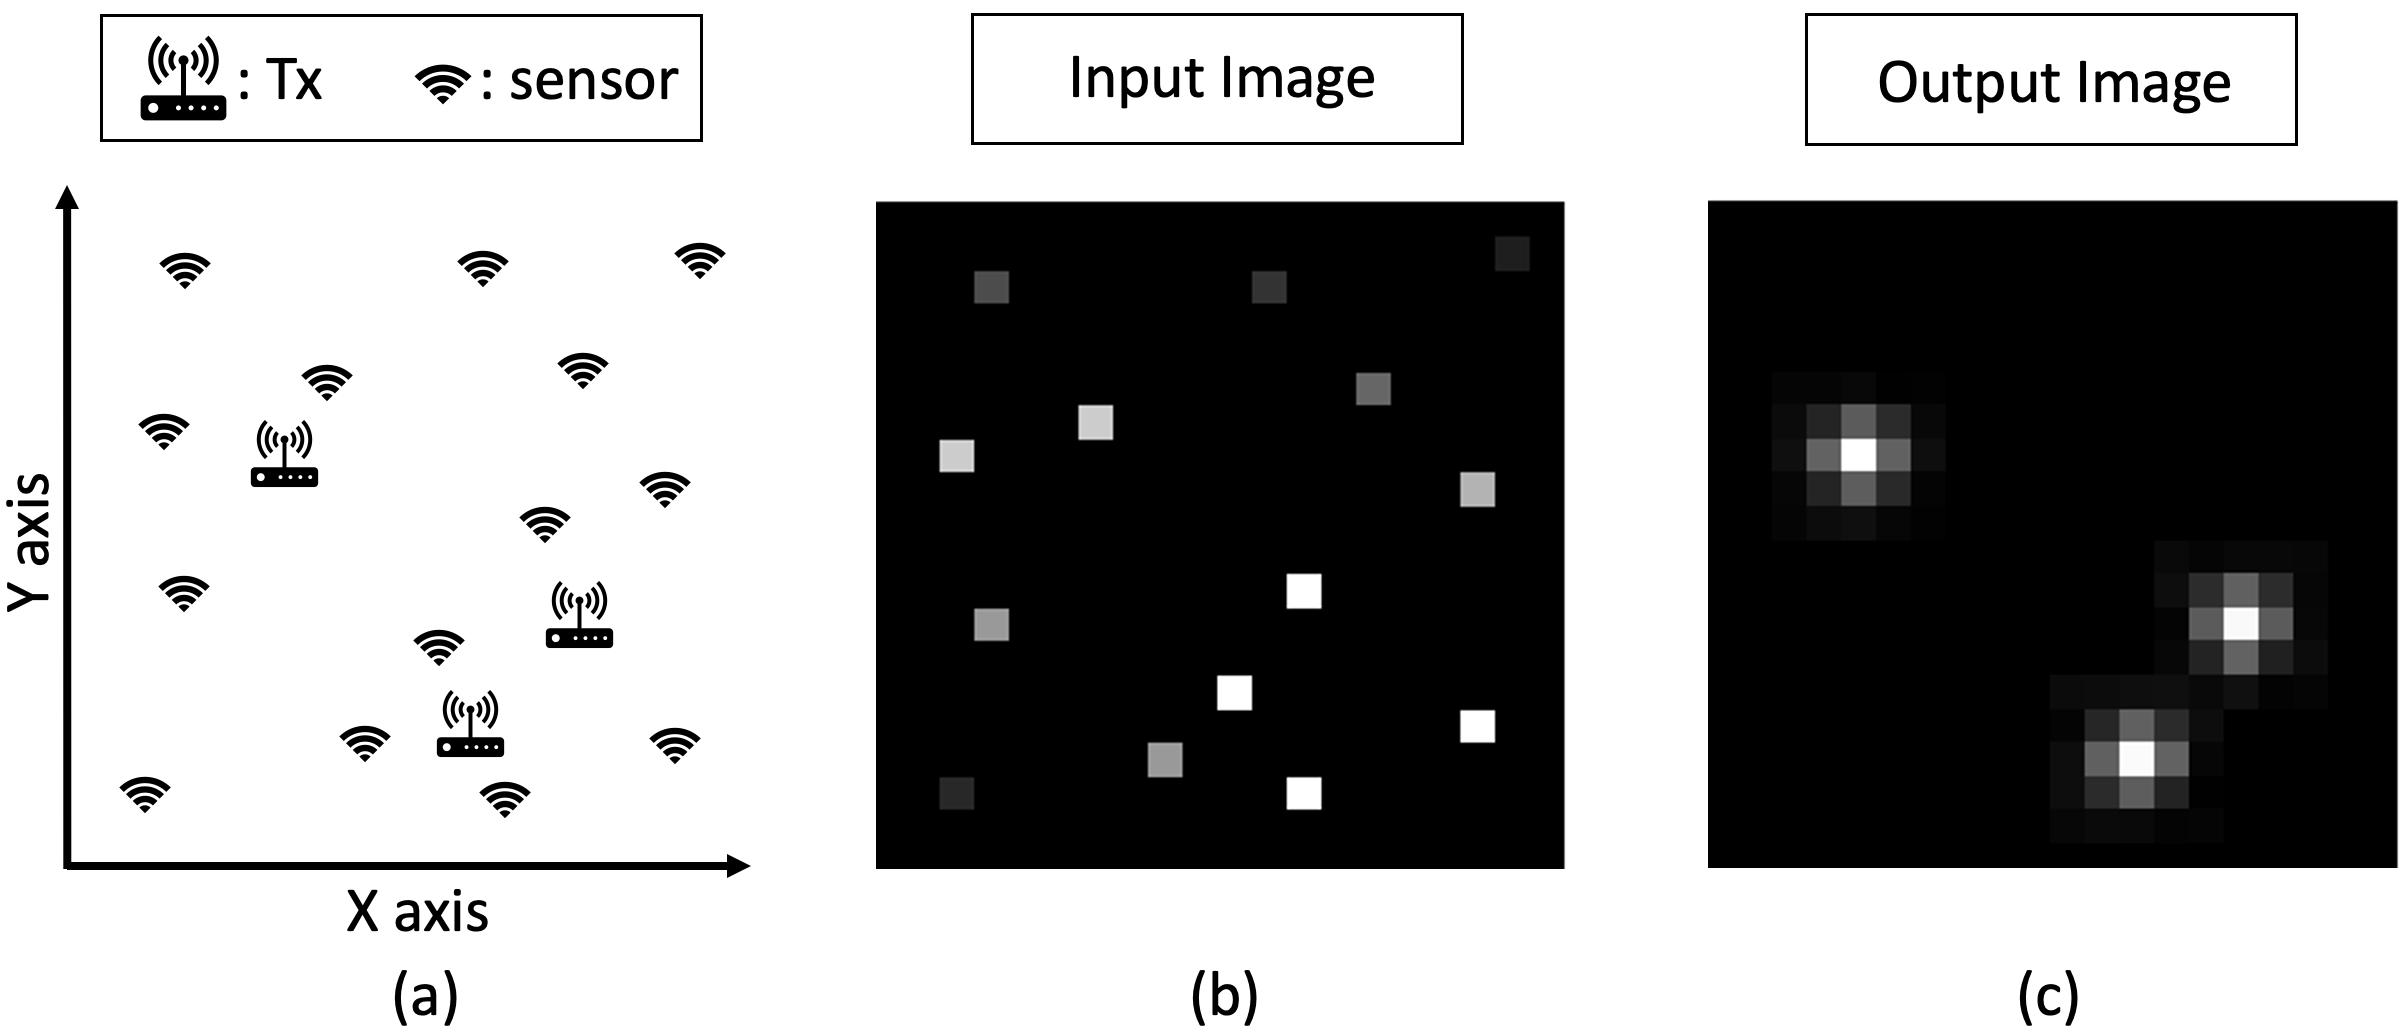
\includegraphics[width=0.8\textwidth]{chapters/wowmom-pmc/figures/input-output.png}
    \caption{Illustration of \our first step's input and output images. (a) Area with distributed sensors and transmitters to be localized. (b) Input image representing the sensor readings (RSS) and locations. (c) Output Image, where we put a 2D Gaussian distribution with its ``peak" at the transmitter's location.}
    \label{fig:input}
\end{figure}
Different than~\cite{mobicom17-splot,ipsn20-mtl}, we represent the sensor information, i.e.,
their locations and observations, in a 2D input image.
%%%%%%%%%%%%%%%%%%%%%%%%%%%%%
We use a 2D grayscale image, and let us denote it $\mx$. The pixel \mxij denotes the observation of the sensor at the grid cell whose index is $(i, j)$. For example, $\mx_{10, 20}=-50$ denotes there is a sensor at coordinate $(10, 20)$ with an RSS reading of $-50$ dB. 
If there is no sensor at location $(i, j)$, we assign the noise floor $\nf$ (i.e. -80 dB) value to \mxij.
Note that the above pixel values (representing the sensor observations) are not the standard
image pixel values that lie in the [0, 255] range.
Also, since the pathloss computed by propagation models during simulations could be real numbers, the sensor observation values could be real numbers. 
So we use a 2D matrix with real numbers instead of an image object.

Before passing this sensor reading image as input to our CNN model, we do a normalization step; we first subtract the $\nf$ from each value and then divide it by $-\nf$/2.
Let $\mxx$ denote the 2D matrix after the normalization of $\mx$. 
The value $\mxxij$ will be zero at locations without sensors, and \mxxij will be a positive real number (in most cases, less than two) for locations with sensors. E.g., if $\mx_{10, 20}=-50$, then the 
$\mxx_{10, 20}$ equals to $(-50- (-80)) / 40) = 0.75$.
Fig.~\ref{fig:input}~(b) shows how a matrix is used to represent the input information that contains both the RSS and the spatial location of the distributed sensors in an area that exists 14 sensors in Fig.~\ref{fig:input}(a).
%%%%%%%%


%%%%%%%%%%%%%%%%%
% \blue{
% When the input is an image, the door of a type of deep learning networks, convolutional neural network (CNN), opens to us. 
% Thus we are able to borrow brilliant new methodologies from the computer vision community.
% }



%%%%%%%%%%%%%%%%%%%%%%%%%%%%%%%%%%%%%%%5

\subsection{Output Image Representing TX locations' Distributions}
\label{subsec:imgimg_output_image}
We now focus on designing the output image to represent the distribution of TX locations; 
the output image is essentially the ``label" assigned to each input image that guides the training of the CNN model. 
Fig.~\ref{fig:input}(c) illustrates the output image of the image-to-image translation step in Fig.~\ref{fig:input}(a) that contains three transmitters.

A straightforward representation that represents the TXs with locations is to just
use an array of $(x, y)$ elements where each $(x, y)$ element is the location of a 
transmitter, as in~\cite{icccn20-deeptxfinder}.
%%%%%%%%%%%%%%
However, this simple representation is less conducive to efficient model learning,
as the representation moves away from spatial representation (by representing locations 
as positions in the image) to direct representation of locations by coordinate values.
E.g., in~\cite{icccn20-deeptxfinder}'s CNN-based approach to \mtl problem, the authors
assume a maximum number $N$ of transmitters and train as many as $N+2$ different CNN models
and thus, limiting the overall solution to the pre-defined maximum number of 
transmitters.
%%%%%%%%%%%%%%
Instead, in our approach, we facilitate the learning of the overall model, by solving the
\mtl problem in two steps, and in this step of translating sensors' reading
to transmitter locations' distributions, we represent the output also as an image.
This approach allows us to use a spatial learning model (e.g. CNN) for the second step too, and preclude
use of regression or fully-connected layers in the first step. 

Inspired by recent work on wireless localization problem~\cite{mobicom20-deeploc} that represents the input and output as images, we represent our output of the first step as an image as well.
The output image is a grayscale image implemented as a 2D matrix with real numbers. 
In the output image, we use 25 ($5\times 5$) pixel values to represent the presence of a transmitter. 
It is desirable to use an odd side length square (e.g., $3\times 3$, $5\times5$, $7\times 7$) for symmetry. 
For a $100\times 100$ size input we use, while $3\times3$ gives too little information for a transmitter and $7\times 7$ generates too many overlaps for close by transmitters, $5\times 5$ is the sweet spot.
Other pixels far away from any transmitter are zero-valued.
%%%%%%%%%%%%%%%%%%%%
Among multiple potential ways to represent a transmitter presence by a number of pixels, we found
that using a 2D Gaussian distribution around the pixel of TX location, as shown in Fig.~\ref{fig:input}(c), yields the best model performance.
Thus, a geographic area with multiple transmitters present is represented by a grayscale image with multiple Gaussian distributions, with each Gaussian distribution's peak inside the pixel corresponding to transmitter's location. 
%%%%%%%%%%%%%%%%%%%%
Based on preliminary performance
tests, we pick the amplitude of the 2D Gaussian peak to 10, the standard deviation to 0.9, and located the center of the distribution at the location of each transmitter.
Note that the location of the TX is in continuous domain and usually not at the center of the grid cell.
%To represent off-center location of a transmitter within the grid cell, we offset the intensity value at each pixel by the distance between the actual location of the transmitter and the grid cell's center.

% \red{Need very precise details. 
% How is the continuous location of TX represented? How many pixels do you use to represent a single TX? How is the power being represented? Note that the transmitter's location is in the continuous domain. 
% So the center of the Gaussian peak is also in the continuous domain, and is usually not precisely located at the center of a pixel. 
% But each pixel is represented as the center of the pixel. 
% Thus the pixel's center value in the 2D Gaussian function will be assigned to the pixel.}

%%%%%%%%%%%%%%%%%%%%%%%%%%%%%%%%%%%%%%%
%%%%%%%%%%%%%%%%%%%%%%%%%%%%%%%%%%%%%%%%

\begin{figure}
    \centering
    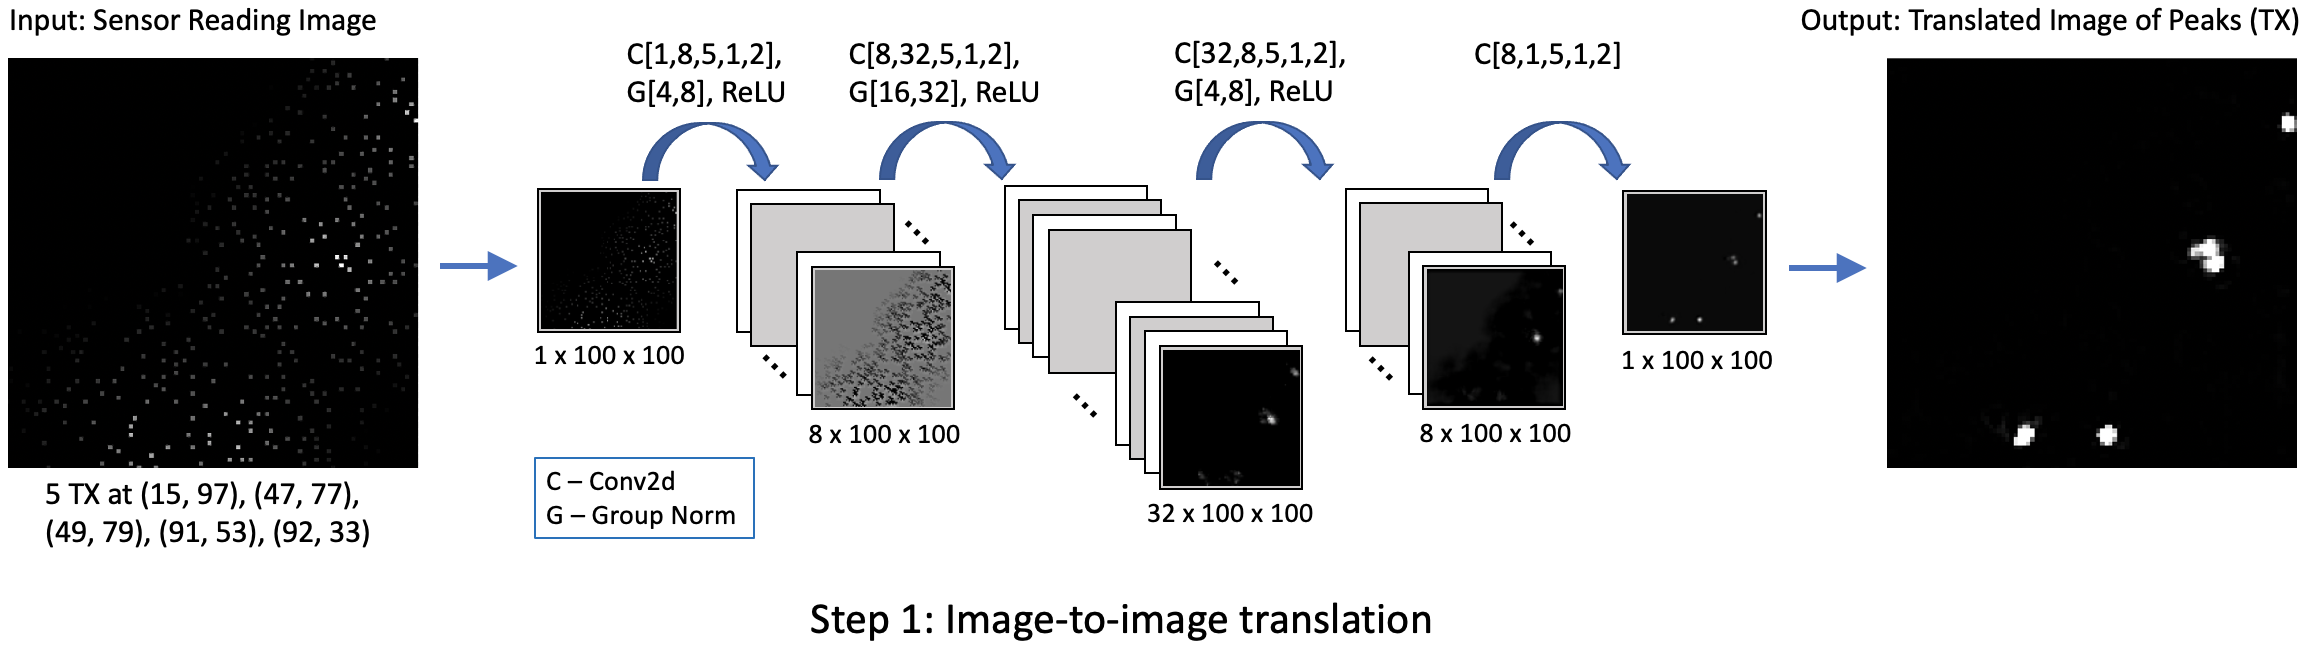
\includegraphics[width=\textwidth]{chapters/wowmom-pmc/figures/part1.png}
    \caption{Architecture of the first step CNN, a four layer image-to-image translation model (\imgimg). The figure displays how the data volume flows through the various convolutional layers. C stands for Conv2d, and for each Conv2d layer, the five values shown are [number of input channels, number of output channels, kernel size, stride, padding]. G stands for group normalization, and, for each group normalization, the two values shown are [number of groups, number of channels]. See~\S\ref{sec:translate} for details.}
    \label{fig:part1}
\end{figure}


\subsection{Image-to-Image Translation: \imgimg CNN Model}
\label{subsec:img-translate}

At a higher level, we use a deep and spatial neural network, in particular a CNN, to learn the
approximation function that maps the input image (of sensor readings) to the output image (of Gaussian distributions for TX locations). We refer to this as the {\em image-to-image translation}
model. Our approach is inspired by the recent work~\cite{mobicom20-deeploc} that frames 
a different wireless localization problem as an image-to-image translation problem.
%%%%%%%
We incorporate the idea into our multiple transmitter localization problem and utilize recent advances in the computer vision area. 
Encoder-decoder based CNN models like U-Net~\cite{miccai15-unet} with down-sampling
and up-sampling convolutional layers have been successful in effectively learning image-to-image translation functions. However, in our setting, we observe that the usage of down-sampling layers (such as max-pooling) degrades the performance of the model, especially in the case when transmitters may be close to each other wherein the model is unable to distinguish the nearby transmitters and generate a single large distribution in the output image. To circumvent this, we avoid using any
down-sampling layers in our model and redesign the image-to-image translation model as described below.

% There are several \red{well-known} learning models that learn functions for image-to-image translation. 
% These image translation models can roughly be classified into two types\cite{img2img-survey}: encoder-decoder-based, such as U-Net~\cite{miccai15-unet}, and GAN-based\cite{nips14-gan}, such as pix2pix~\cite{cvpr17-pix2pix}. In general, GAN-based models 
% are more  complex than the encoder-decoder-based models, and \red{their goal is vastly different than ours .... some specific details as to why GAN-based are not relevant for us.} 
%%%%%%%%%%%%%
% For our context, wherein our target images are much simpler, we observe that the simple encoder-decoder image translation model is sufficient to solve our problem. 
%%%%%%%%%%%%%%%%%
% \red{Describe some high-level differences between GAN and encoder-decoder models, or at the very least, what the encoder-decoder model looks like.}
%%%%%%%%%%%%%%%%%%%%%%%
% We tried standard encoder-decoder model design strategies and \red{HG: The following sentences can not be understood, without more details on encoder-decoder modes.} skip connections like \cite{miccai15-unet}. But we found out that the down-sampling mechanisms such as max-pooling are losing the information and the skip connection are not enough to make up the information loss.

\para{\imgimg CNN Model}. 
We refer to our image-to-image translation CNN model as \imgimg, as it translates sensors' 
readings to ``peaks" with Gaussian distributions corresponding to transmitter locations.  
It has four \footnote{We observe that a four-layer lightweight and symmetric \imgimg  model produces good results and adding more layers gives marginal improvement.}
convolutional layers, as shown in Fig.~\ref{fig:overall}(a). 
We use an input size of $100\times100$. The number of convolutional filters are varying for
different layers, with up to 32 in one of the layers. 
%%%%%
We tried doubling the filter numbers at each layer, but it does not lead to significant 
improvement (it does yield a lower error, but the output image does not improve significantly
to impact the second step of our architecture). We use a kernel size of $5\times5$, a stride of 1, and a padding of 2.
This ensures that the dimensions do not decrease and all the pixels are treated 
uniformly, including the ones at the edge of the image.
With the above four convolutional layers, the receptive field~\cite{receptive-field} of each neuron in the output layer is $17\times17$.
Normalization layers can improve the learning process. We chose group normalization \cite{groupnorm} and put it after the first three convolutional layers. 
We compared group and batch normalization~\cite{batchnorm} methods in our context, and observed
better performance with the group normalization. 
For the activation layers, we select rectified linear unit (ReLU) and put it after the group normalization layers.

% \softpara{Derived Pixels in Higher Layers.} 
% We have four convolutional layers with kernel size of 5x5. 
% So a neuron on the first convolutional layer will have 
% 5x5 view of the input volume, and a neuron on the second convolutional layer will have a 5x5 view of the first convolutional layer and thus a 9x9 view of the input volume, and so on. Thus, a 
% a neuron on the forth convolutional layer (and also the output layer) 
% will have a 17x17 view of the input volume. So each single pixel 
% in the output image is derived from 17x17 pixels of the input image. \blue{Whats the point of talking about this? .}

\softpara{The Loss Function}. Our inputs ($X$) and output ($Y$) are images. We use L2 loss function which computes the mean squared error aggregated over individual pixels.
More formally, our loss function is  defined as:
\begin{equation}
 \frac{1}{N} \sum_{i}^{N} || \imgimg(X_i) - Y_i ||^2
 \label{equ:sen2peak_loss}
\end{equation}
where $N$ is the number of samples used in computing the loss, $|| \cdot ||^2$ is L2 loss function, $X_i$ and $Y_i$ are the $i_{th}$ sample's input and output images respectively, and $\imgimg(X_i)$ is the predicted output image corresponding to the input $X_i$. During training, we use 
Adam~\cite{kingma2017adam} as the optimizer that minimizes the loss function. We set the learning rate to 0.001 and the number of epochs to 20 and the model converges well.
% \red{more info about the training and testing such as normalization. HG: Not sure its needed.}